\documentclass[12pt]{beamer}
%\usepackage[left=3cm, right=1.5cm, top=2cm, bottom=2cm]{geometry}
%\usepackage[T2A]{fontenc}
%\usepackage{cmap}
\usepackage[utf8]{inputenc}
\usepackage[english,russian]{babel}
\usepackage{indentfirst}
\usepackage{amsmath}
\usepackage{amssymb}
\usepackage{graphicx}

\usepackage{hhline}
\usepackage{longtable}
\usetheme{Singapore}

\renewcommand{\figurename}{Рисунок}
\begin{document}
\title{\small{Реализация библиотеки параллельной записи больших файлов с вещественными числами в текстовом представлении}}
\author{Нагорных Яна}
\date{\footnotesize{Москва -- 2018}}
\frame{
\begin{center}
\footnotesize{МГУ имени М. В. Ломоносова}\\
\footnotesize{Механико-математический факультет}\\\vspace{28pt}
\small Презентация к курсовой работе \\
\end{center}
\titlepage
} 
\section{Введение}
\frame{
Печать больших массивов чисел без округления с большой точностью всегда занимает много времени.
Однако, не вся печать упирается в возможности диска, как это может показаться.
Кроме того, у печати данных мало ресурсов для ускорения.\\
\vspace{14pt}
\textbf{Цели работы:}
\begin{enumerate}
\item Ускорить печать больших массивов без потери точности;
\item Использовать быстрые алгоритмы печати целых чисел и чисел с плавающей точкой.
\end{enumerate}
}
\frame{
\textbf{Возможные варианты улучшений:}
\vspace{14pt}
\begin{itemize}
\item Применение более быстрых алгоритмов преобразования чисел в строки
\vspace{14pt}
\item Использование многопоточного программирования
\vspace{14pt}
\item Изменение формата вывода (отбрасывание лишних нулей, сокращенная запись повторяющихся чисел)
\end{itemize}
}

\section{Описание алгоритма}
\frame{
\textbf{Распределение задач}\\
Наглядно работа потоков изображена на рисунке:
\begin{figure}[h!]
\begin{tiny}
\def\svgwidth{300pt}
  \input{pics/drawing.pdf_tex}
\end{tiny}\end{figure}
}
\frame{
\textbf{Алгоритм Grisu}\\
\begin{itemize}
\item Выражаем $v$: $$v=\cfrac{f_v}{2^{-e_v}}.$$
\item Десятичные цифры $v$ могут быть вычислены путем нахождения десятичного показателя $t$, для которого $$1 \leqslant \cfrac{f_v \times 10^t}{2^{-e_v}} < 10$$.
\item Идея \textsf{Grisu} состоит в кэшировании приблизительных значений дробей $\cfrac{10^t}{2^{e_t}}$.
\end{itemize}
}
\frame{
\textbf{Алгоритм Grisu2}\\
\vspace{14pt}
\begin{itemize}
\item У \textsf{Grisu} есть существенный недостаток.
Например, при значениях по умолчанию число 1 будет напечатано в виде \texttt{10000000000000000000e-19.}
\vspace{14pt}
\item В отличие от \textsf{Grisu} алгоритм \textsf{Grisu2} не генерирует полное десятичное представление, а просто возвращает значащие цифры и соответствующий показатель. 
Затем процедура форматирования объединяет эти данные для получения представления в требуемом формате.
\end{itemize}
}
\frame{
\begin{itemize}
\item \textsf{Grisu2} использует дополнительные флаги для создания более короткой выходной строчки. 
\vspace{14pt}
\item Также \textsf{Grisu2} не будет работать с точными числами, а вместо этого будет вычислять аппроксимации $m^{-}$ и $m^+$ -- \textit{ближайшие числа в памяти}.
\vspace{14pt}
\item Во избежание ошибочных результатов, увеличивается диапазон, в котором, согласно алгоритму, может оказаться полученное число.  
\end{itemize}
}
\frame{
\begin{small}
\begin{figure}[h!]
\begin{center}
\texttt{ 
\begin{tabular}{|l|c|l|}
\hhline{|-|~|-|}
  array[0] = 1;				& & 1 \\
  array[1] = 1.2;			& & 1.2 \\
  array[2] = 1.23;			& & 1.23\\
  array[3] = 1.23400000;			& & 1.234 \\
  array[4] = 1.23456789;	& & 1.23456789\\
  array[5] = -1;			& & -1\\
  array[6] = -1.234;		& $\longrightarrow$ & -1.234\\
  array[7] = sqrt (2);		& & 1.4142135623730952\\
  array[8] = 1234e-36;		& & 1.234e-33\\
  array[9] = 0.000000123;	& & 1.23e-7\\
  array[10] = 0.123;		& & 0.123\\
  array[11] = 12.3;	& & 12.3\\
  array[12] = 123.000;	& & 123\\
\hhline{|-|~|-|}
\end{tabular}
}
\textit{ 
\begin{tabular}{ccc}
$\qquad\quad$ массив $\qquad\quad$ & $\qquad\qquad$ & выходной файл \\
\end{tabular}
}
\end{center}
\end{figure}
\end{small}
}
\frame{
\textbf{Улучшения}\\
\vspace{14pt}
\begin{itemize}
\item Если в массиве есть $n$ подряд идущих одинаковых чисел с заданной точностью, то есть $\forall i: \, 1 \leqslant i < n$ верно, что $\|x_i - x_{i-1}\| \leqslant \varepsilon$, то сократим запись $n$ чисел и вернем строку вида \texttt{n*x}.
\vspace{14pt}
\item
Запись целых чисел, означающих количество повторяющихся элементов массива, также можно ускорить.
Суть алгоритма заключается в быстром логарифмировании числа по основанию 10.
\end{itemize}
}
\section{Результаты работы}
\frame
{
\textbf{Случайные числа}
\begin{footnotesize}
\begin{center}
\begin{longtable}{||c|c|c|c|c|c|c||}
\hline
\hline
Размер & \multicolumn{4}{c|}{Число потоков} & Стандартная & Размер\\
\hhline{~|-|-|-|-|~|~|}
массива & 6 & 4 & 2 & 1 & печать &файла\\
\hline
\hline
 & 0.593 & 0.880 & 1.620 & 3.196 & 4.256 & \\
\hhline{~|-|-|-|-|-|~|}
$10^7$   & 0.562 & 0.841 & 1.612 & 3.239 & 4.176 & 245 MB \\
\hhline{~|-|-|-|-|-|~|}
 & 0.530 & 0.802 & 1.502 & 3.052 & 4.188 &\\
\hline
&2.571& 4.044 & 7.812 & 15.37 & 22.47 & \\
\hhline{~|-|-|-|-|-|~|}
$5 \cdot 10^7$  & 2.634 & 4.273 & 8.214 & 16.30 & 21.11 &  1.2 GB\\
\hhline{~|-|-|-|-|-|~|}
 & 2.689 & 4.179 & 7.822 & 15.32 & 20.89 & \\
\hline
 & 5.219 & 8.276 & 15.67 & 32.46 & 41.71 & \\
\hhline{~|-|-|-|-|-|~|}
$10^8$  & 5.077 & 7.970 & 15.30 & 30.57 & 41.78 & 2.4 GB\\
\hhline{~|-|-|-|-|-|~|}
& 5.189 & 8.078 & 15.37 & 30.75 & 41.96 & \\
\hline
 & 41.12 & 49.15 & 75.23 & 148.91 & 200.94 & \\
\hhline{~|-|-|-|-|-|~|}
$5 \cdot 10^8$ & 40.23 & 50.08 & 75.92 & 149.08 & 200.33 & 12 GB\\
\hhline{~|-|-|-|-|-|~|}
 & 41.23 & 49.16 & 74.92 & 148.52 & 200.69 & \\
\hline
\hline
\end{longtable}
\end{center}
\end{footnotesize}
}
\frame{
Среднее ускорение работы алгоритма:
\begin{center}
\begin{tabular}{||c|c|c|c|c||}
\hline
\hline
Размер & \multicolumn{4}{c||}{Число потоков}\\
\hhline{~|-|-|-|-|}
массива & 6 & 4 & 2 & 1 \\
\hline
$10^7$ &  7.49  & 5.00 & 2.67 & 1.33 \\
\hline
$5 \cdot 10^7$ & 8.17 & 5.16 & 2.70 & 1.37 \\
\hline
$10^8$ & 8.10 & 5.16 & 2.71 & 1.34\\
\hline
$5 \cdot 10^8$ & 4.91 & 4.06 & 2.66 & 1.35\\
\hline
\hline
\end{tabular}
\end{center}
Ускорение на одном потоке демонстрирует ускорение работы \textsf{Grisu2} по сравнению со стандартной печатью.
}
\frame{
Наглядно зависимость времени от числа потоков для массива размером $10^8$ изображена на графиках.
\begin{figure}[h!]
\begin{minipage}[h]{0.45\linewidth}
\center{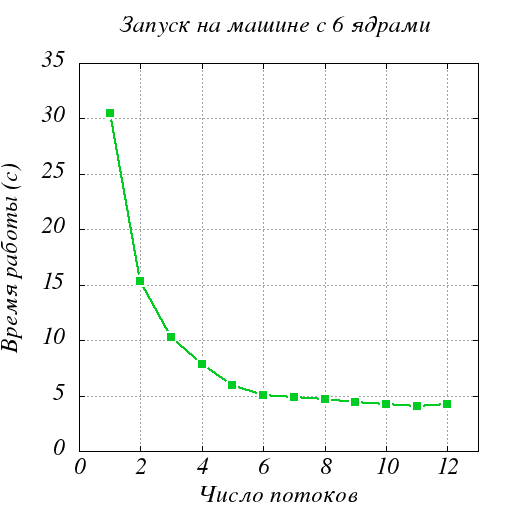
\includegraphics[width=1\linewidth]{./pics/time.png}}
\end{minipage}
\hspace{5pt}
\begin{minipage}[h]{0.45\linewidth}
\center{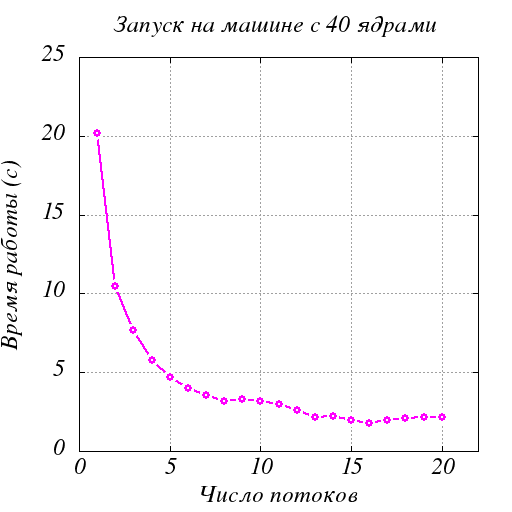
\includegraphics[width=1\linewidth]{./pics/time40.png}}
\end{minipage} 
\end{figure}
}
\frame{
\textbf{Целые числа}
\begin{footnotesize}
\begin{center}
\begin{longtable}{||c|c|c|c|c|c|c||}
\hline
\hline
Размер & \multicolumn{4}{c|}{Число потоков} & Станд. & Размер\\
\hhline{~|-|-|-|-|~|~|}
массива & 6  & 4 & 2 & 1 & печать & файла\\
\hline
\hline
 & 0.213 & 0.322 & 0.643 & 1.297 & 5.300  &\\
\hhline{~|-|-|-|-|-|}
$10^7$ & 0.216 & 0.320 & 0.649 & 1.284 & 5.245  &56 MB / 205 MB \\
\hhline{~|-|-|-|-|-|}
 & 0.219 & 0.337 & 0.650 & 1.321 & 5.312  &\\
\hline
& 1.052 & 1.664 & 3.319 & 6.362 & 27.93  &\\
\hhline{~|-|-|-|-|-|}
$5 \cdot 10^7$& 1.069  & 1.675 & 3.334 & 6.375 & 29.46  &295 MB / 1 GB\\
\hhline{~|-|-|-|-|-|}
& 1.071  & 1.662 & 3.340 & 6.490 & 29.43  &\\
\hline
 & 2.057 &  3.374 & 6.618 & 12.61 & 55.04 & \\
\hhline{~|-|-|-|-|-|}
$10^8$ & 2.018 & 3.309 & 6.712 & 12.63 & 55.70  & 590 MB / 2 GB \\
\hhline{~|-|-|-|-|-|}
 & 2.012 & 3.248 & 6.601 & 13.66 & 56.31  &\\
\hline
 & 10.82 & 16.68 & 32.14 & 62.94 & 283.61  &\\
\hhline{~|-|-|-|-|-|}
$5 \cdot 10^8$ & 10.91 & 16.68 & 32.20 & 64.08 & 290.70  &2.9 GB / 10 GB\\
\hhline{~|-|-|-|-|-|}
 & 10.15 & 16.45 & 32.09 & 64.12 & 287.54  &\\
\hline
\hline
\end{longtable}
\end{center}
\end{footnotesize}
}
\frame{
Размер файла, полученного с помощью нового алгоритма гораздо меньше размера файла, полученного стандартной печатью, так как отброшены лишние нули.
За счет этого ускорение возросло:
\begin{center}
\begin{tabular}{||c|c|c|c|c||}
\hline
\hline
Размер & \multicolumn{4}{c|}{Число потоков}\\
\hhline{~|-|-|-|-|}
массива & 6 & 4 & 2 & 1 \\
\hline
$10^7$  & 24.47  & 16.19 & 8.17 & 4.06 \\
\hline
$5 \cdot 10^7$ & 27.20 & 17.36& 8.69 & 4.51 \\
\hline
$10^8$ & 27.44 & 16.82 & 8.38 & 4.29 \\
\hline
$5 \cdot 10^8$ & 27.03  & 17.30 & 8.93& 4.51 \\
\hline
\hline
\end{tabular}
\end{center}
}
\frame{
\textbf{Повторяющиеся числа}
\begin{footnotesize}
\begin{center}
\begin{longtable}{||c|c|c|c|c|c|c||}
\hline
\hline
Размер & \multicolumn{4}{c|}{Число потоков} & Станд. & Размер \\
\hhline{~|-|-|-|-|~|~|}
массива & 6 & 4 & 2 & 1 & печать  & файла\\
\hline
\hline
& 0.112 & 0.181 & 0.339 & 0.652 & 3.445  &\\
\hhline{~|-|-|-|-|-|}
$10^7$ & 0.109 & 0.159 & 0.310 & 0.604 & 3.322  & 24 MB / 187 MB \\
\hhline{~|-|-|-|-|-|}
& 0.119 & 0.168 & 0.329 & 0.661 & 3.460  &\\
\hline
& 0.521 & 0.843 & 1.630 & 2.983 & 16.91  &\\
\hhline{~|-|-|-|-|-|}
$5 \cdot 10^7$ & 0.549 & 0.841 & 1.643 & 3.067 & 17.30  & 123 MB / 936 MB\\
\hhline{~|-|-|-|-|-|}
& 0.530 & 0.833 & 1.612 & 2.875 & 16.96 & \\
\hline
& 1.178 & 1.748 & 3.343 & 6.056 & 36.19 &\\
\hhline{~|-|-|-|-|-|}
$10^8$ & 1.152 & 1.678 & 3.209 & 5.959 & 36.38  & 245 MB / 1.8 GB\\
\hhline{~|-|-|-|-|-|}
& 1.163 & 1.689 & 3.290 & 6.039 &  36.41  &\\
\hline
& 5.720 & 8.354 & 15.82 & 31.50 & 182.22 &\\
\hhline{~|-|-|-|-|-|}
$5 \cdot 10^8$ &5.714 & 8.346 & 15.71 & 31.29 & 182.00  & 1.2 GB / 9.4 GB\\
\hhline{~|-|-|-|-|-|}
& 5.816 & 8.418 & 15.92 & 31.69 & 183.52  &\\
\hline
\hline
\end{longtable}
\end{center}
\end{footnotesize}
}
\frame{
За счет того, что все последовательности одинаковых подряд идущих чисел будут сворачиваться в короткую строку вида \texttt{n*x}, уменьшился файл и увеличилось ускорение.
\begin{center}
\begin{tabular}{||c|c|c|c|c||}
\hline
\hline
Размер & \multicolumn{4}{c|}{Число потоков}\\
\hhline{~|-|-|-|-|}
массива & 6 & 4 & 2& 1 \\
\hline
$10^7$  & 30.08 & 20.13 & 10.46 & 5.33 \\
\hline
$5 \cdot 10^7$ & 31.98 & 20.32 & 10.47 & 5.74 \\
\hline
$10^8$ & 31.20 & 21.31 & 11.07 & 6.03 \\
\hline
$5 \cdot 10^8$ & 31.75 & 21.81 & 11.54 & 5.80 \\
\hline
\hline
\end{tabular}
\end{center}
}
\frame{
\textbf{Огромные массивы случайных чисел}\\
\begin{itemize}
\item Сравним стандартную печать и алгоритм, запущенный на 12 (+2) потоках.
\item Помимо обычного запуска, проведем и запуск с записью не на диск, а в разделяемую память \textit{shared-memory}.
\item На следующем графике приведена зависимость времени работы от размера массива.
\end{itemize}
}
\frame{
\begin{figure}[h!]
\center{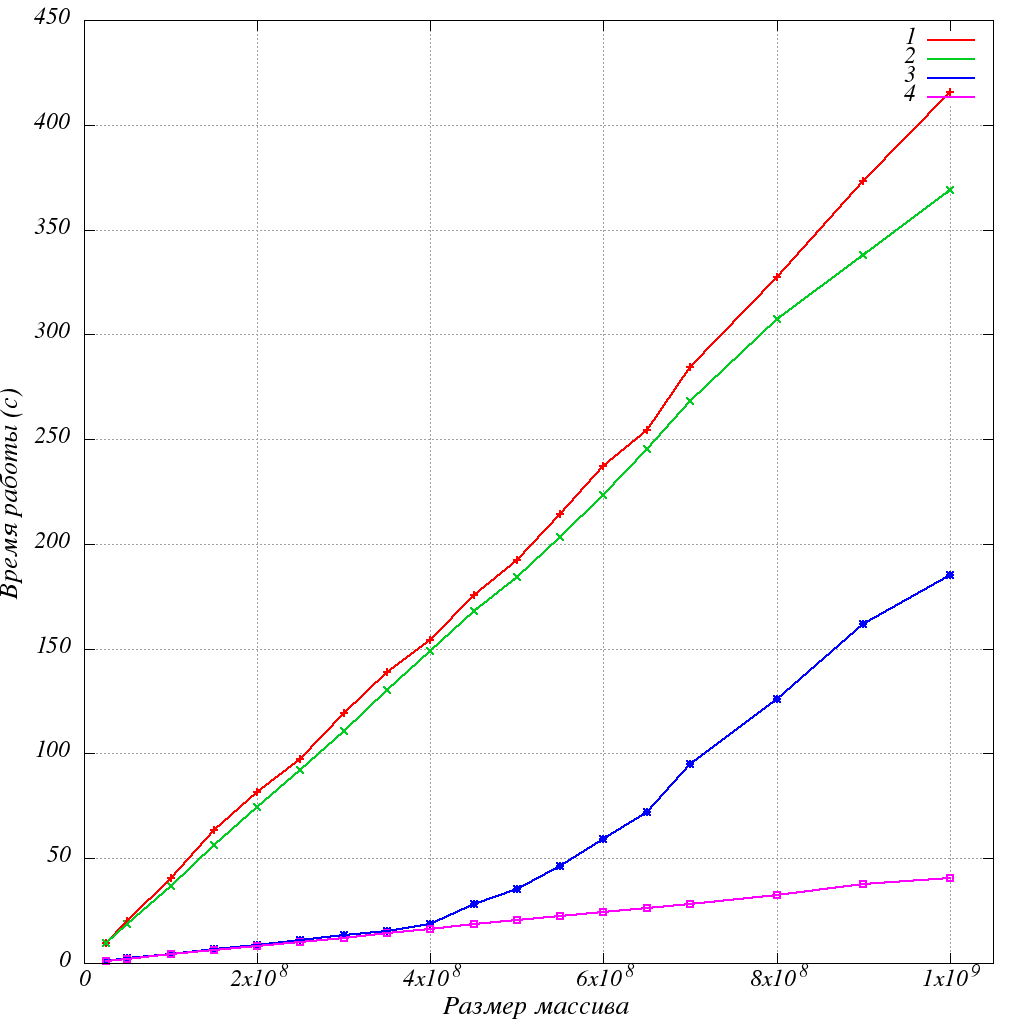
\includegraphics[width=0.65\linewidth]{./pics/graphics.png}}
\end{figure}
\tiny
{
1 -- стандартная печать с записью на диск;
2 -- стандартная печать с записью в разделяемую память;
3 -- алгоритм параллельной печати с записью на диск;
4 -- алгоритм параллельной печати с записью в разделяемую память.}
}
\section{Заключение}
\frame{
\begin{itemize}
\item В результате написания курсовой работы была решена поставленная задача: 
реализована библиотека параллельной записи массивов вещественных чисел.
\item В ходе тестирования была проверена точность работы реализованного алгоритма, а также измерено ускорение в сравнении со стандартной функцией печати. 
\item Написанная на языке \textsf{С++} подпрограмма была внедрена в промышленный гидродинамический симулятор \textsf{tNavigator}.
\end{itemize}
}
\frame{
\textbf{Список использованной литературы}
\begin{thebibliography}{}
\bibitem{1} \textsc{Florian Loitsch}.
Printing Floating-Point Numbers Quickly and Accurately with Integers, 2004.
\bibitem{2} \textsc{Wojciech Mu\l a}.
SSE: conversion integers to decimal representation, 2011.
\bibitem{3} \textsc{Богачев К.Ю.}.
Основы параллельного программирования. -- M.: Бином. Лаборатория знаний, 2010.
\bibitem{4} \textsc{David Goldberg.}
What every computer scientist should
know about floating-point arithmetic. -- ACM Computing Surveys, 23(1): 5–48, 1991.
\end{thebibliography}
}
\frame{
\begin{center}
\Huge{Спасибо за внимание!}
\end{center}
}
\end{document}